\documentclass[a4paper,11pt]{article}

\usepackage[utf8]{inputenc}
\usepackage[english]{babel}

\usepackage{amsmath}

% Code highligting
% \usepackage{minted}
\usepackage[outputdir=output/tex]{minted} % iom min makefile

\newenvironment{longlisting}{\captionsetup{type=listing}}{}
% \renewcommand\listoflistingscaption{Källkod....}
\renewcommand\listoflistingscaption{List of source codes}
%\setmintedinline[sql]{breaklines=true,breakanywhere=true} % necessary for breakanywhere to work later on.

\usepackage{graphicx}
\usepackage{pgf}
\usepackage{wrapfig}
\usepackage[font=footnotesize,labelfont=bf,skip=1pt]{caption}
\usepackage{subcaption}

\usepackage{pgfplots}
\pgfplotsset{compat=1.18}

\usepackage{pgfplotstable}
\usepackage{booktabs}

% Spacing
\usepackage{titlesec}
%\titlespacing*{\section}{0pt}{2ex plus 1ex minus .2ex}{1ex plus .2ex}
%\titlespacing*{\subsection}{0pt}{1ex plus 1ex minus .2ex}{1ex plus .2ex}

\usepackage{hyperref}

\begin{document}

\title{
    An environment
\\\small{Programmering II, ID1019, VT24 P1}
}
\author{Vincent Ferrigan \href{mailto:ferrigan@kth.se}{ferrigan@kth.se}}

% \date{\today}
\date{Spring Term 2023}

\maketitle

\section*{Introduction}
\label{sec:introduction}
The objective of this assignment is to explore and analyze
the efficiency of
different data structure implementations for storing
and retrieving key-value pairs.
These key-value databases are also referred to as ''maps''.
The first task involves developing two different implementations;
one based on a simple list structure and the
another based on a tree structure.
The latter was implemented as a \emph{Binary Search Tree} (BST).
%A BST is a node-based binary tree data structure where each node has a key and value, and satisfies the BST property: the key in each node must be greater than all keys in the left subtree and less than those in the right subtree.

The second task is to compare these two ''custom implementations'',
both with eachother and, in terms of performance, with
Elixir's built-in Map module.

This assignment is based on the instruction
\href{https://people.kth.se/~johanmon/courses/id1019/seminars/environment/environment.pdf}{'An environment'}
by course examiner Johan Montelius.
The Mix-project for this assignment, including all relative functions, Unit-test and benchmarks can be found on GitHub:
\href{https://github.com/VincentFerrigan/kth-id1019-programming-ii/tree/main/tasks/2/mymaps}{Repo Programming II - My Maps}% TODO FUNKAR DEN? ÄNDRA NAMN

\section*{Methods}
\label{sec:methods}

\subsection*{Literature Study}
\label{subsec:literaturestudy}
The pre-recorded lectures on
\href{https://canvas.kth.se/courses/44911/assignments/syllabus}{Lists, Recursion and Trees},
given by the course examiner, were reviewed.
Elixir-syntax and similar topics were acquired
from both the
\href{https://elixir-lang.org/docs.html}{Elixir official documentation}
and the free Elixir Tutorial
\href{https://elixirschool.com/en}{Elixir School
website}.
The author also relied on textbooks found on
\href{https://learning.oreilly.com}{O'Reilly Media},
especially Brute Tate's
\href{https://learning.oreilly.com/library/view/programmer-passport-elixir/9781680509649/}{Programmer Passport: Elixir}.

\subsubsection*{Tools and packages}
\label{subsec:tools}
All code was written in \emph{IntelliJ IDEA}.
Quick-fixes and editing was, however, done in \emph{Vim}. 
\emph{GIT} and \emph{GitHub} were used for version control.
Tests were performed with Elixir's built-in test framework \emph{ExUnit.}
For the visualization of benchmarking results, \emph{GNUPlot} was used.
This report was also written in plain text mode -- \LaTeX.

\subsubsection*{The overall Work-flow} % \todo BYT NAMN?
\label{subsec:workflow}
%/TODO Är det här jag har med kod?? Eller kör jag det i resultat delen? Annars kanske det enbart räcker med att skriva varje steg för steg.
The development was an iterative approach with ''trail and errors''.
The author practiced
\href{https://www.elixirwiki.com/wiki/Test-Driven_Development_in_Elixir}{Test Driven Development}
(TDD).
The basic steps follow the \emph{Red-Green-Refactor cycle};
writing failing tests (Red), make them pass (Green),
and finally refactor the code.

In addition to the list- and tree-based data structure implementations of map,
a wrapper module (\mintinline{elixir}{MapWrapper}) was developed to provide a
consistent interface for Elixir’s built-in Map,
aligning its
\mintinline{elixir}{put/3},
\mintinline{elixir}{get/2}, and
\mintinline{elixir}{delete/2} functions with the
\mintinline{elixir}{add/3},
\mintinline{elixir}{lookup/2}, and
\mintinline{elixir}{remove/2} functions used in the custom implementations.
\begin{minted}[fontsize=\small]{elixir}
defmodule MapWrapper do
    def new(), do: %{}
    def add(map, key, value), do: Map.put(map, key, value)
    def lookup(map, key), do: Map.get(map, key)
    def remove(map, key), do: Map.delete(map, key)
end
\end{minted}
For the
\href{https://github.com/VincentFerrigan/kth-id1019-programming-ii/blob/main/tasks/2/mymaps/lib/benchmark.ex}{benchmarking module},
Erlangs
\mintinline{elixir}{:timer} module was used to measure the time taken for the
\emph{add}, \emph{lookup}, and \emph{remove} operations.
Both \emph{GNUPlot} and \emph{Python} scrips were used to collect, manipulate and present the results.

\section*{Result}
\label{sec:result}
%\TODO: Här inkluderar du alla benchmarks
Since all
\href{https://github.com/VincentFerrigan/kth-id1019-programming-ii/tree/main/tasks/2/mymaps/lib}{code (.ex)}, % TODO FUNKAR DEN? ÄNDRA NAMN
\href{https://github.com/VincentFerrigan/kth-id1019-programming-ii/tree/main/tasks/2/mymaps/data}{graphs (.png)}, and % TODO FUNKAR DEN? ÄNDRA NAMN
\href{https://github.com/VincentFerrigan/kth-id1019-programming-ii/tree/main/tasks/2/mymaps/data}{tables (.dat)}% TODO FUNKAR DEN? ÄNDRA NAMN
could be found on GitHub, the author has chosen only to present one of the operations; lookup.
However, all operations will be addressed in the \hyperref[sec:discussion]{Discussion} section.
The implementation of the lookup operation for the list-based map can be found in Listing \autoref{listing:EnvList.lookup()}
while the tree-based version can be found in Listing \autoref{listing:EnvTree.lookup()}.
Both return the key with its value as a tuple
\mintinline{elixir}{{key, value}} or
\mintinline{elixir}{:nil} if the key is not found.
\begin{longlisting}
    \belowcaptionskip=5pt
    \inputminted[
        label=Derivative.run/3,
%        linenos=true,
        firstline=54,
        lastline=57,
        xleftmargin=-5mm,  % Adjust this value as needed
%        frame=single,
        fontsize=\small,
    ]{elixir}{../lib/env_list.ex}
    \caption{The implementation of the Lookup operation for list-based maps.}
    \label{listing:EnvList.lookup()}
\end{longlisting}
As one can derive from the code in Listing ~\autoref{listing:EnvTree.lookup()},
the tree-based map is implemented as a BST.
A BST is a node-based binary tree data structure where each node contains a key and its value.
All keys in a nodes left subtree must be less than those in its right subtree.
\begin{longlisting}
    \belowcaptionskip=5pt
    \inputminted[
        label=Derivative.run/3,
%        linenos=true,
        firstline=57,
        lastline=61,
        xleftmargin=-5mm,  % Adjust this value as needed
%        frame=single,
        fontsize=\small,
    ]{elixir}{../lib/env_tree.ex}
    \caption{The implementation of the Lookup operation for tree-based maps}
    \label{listing:EnvTree.lookup()}
\end{longlisting}
The result of the benchmark is illustrated in the figures and table below.
~\autoref{fig:lookup_performance} and ~\autoref{fig:tm_lookup_performance}
diagrammatically visualize the lookup operation while the
data is described in ~\autoref{tab:performance_metrics_and_ratios_lookup}.
    \begin{table}[htbp]
        \centering
        \pgfplotstabletypeset[
        col sep=space, % adjust this based on your .dat file format
        every head row/.style={before row=\toprule, after row=\midrule},
        every last row/.style={after row=\bottomrule},
        columns/Size/.style={column name=Size (n)},
        columns/List/.style={column name=List (\mu s)},
        columns/Tree/.style={column name=Tree (\mu s)},
        columns/Map/.style={column name=Map (\mu s)},
        columns/List:Tree/.style={column name=$\frac{List}{Tree}$},
        columns/List:Map/.style={column name=$\frac{List}{Map}$},
        columns/Tree:Map/.style={column name=$\frac{Tree}{Map}$},
        ]{../data/combined_lookup_ratios.dat}
        \caption{Comparative Performance Metrics and Ratios for the Lookup operation}
        \label{tab:performance_metrics_and_ratios_lookup}
    \end{table}
    \begin{figure}[htbp]
        \centering
        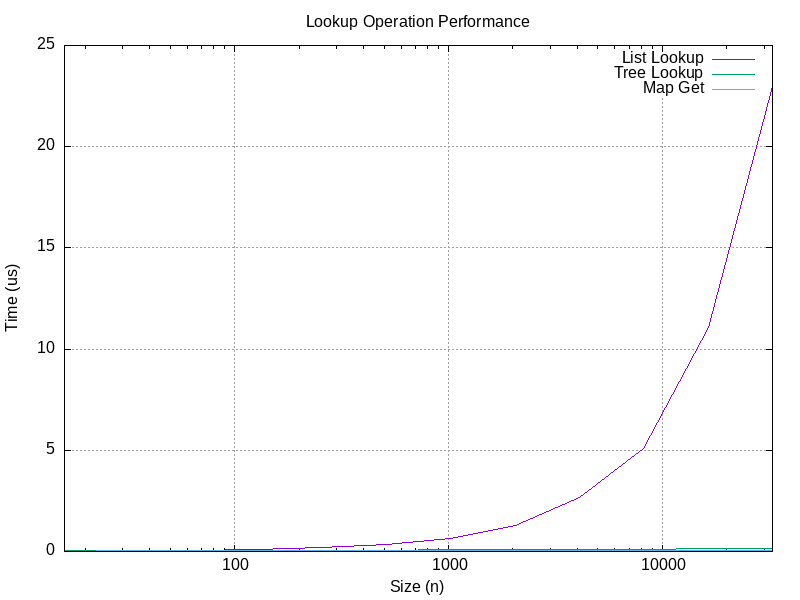
\includegraphics[width=\textwidth]{../data/lookup_performance.png}
        \caption{Lookup Operation Performance}
        \label{fig:lookup_performance}
    \end{figure}

\begin{figure}[htbp]
    \centering
    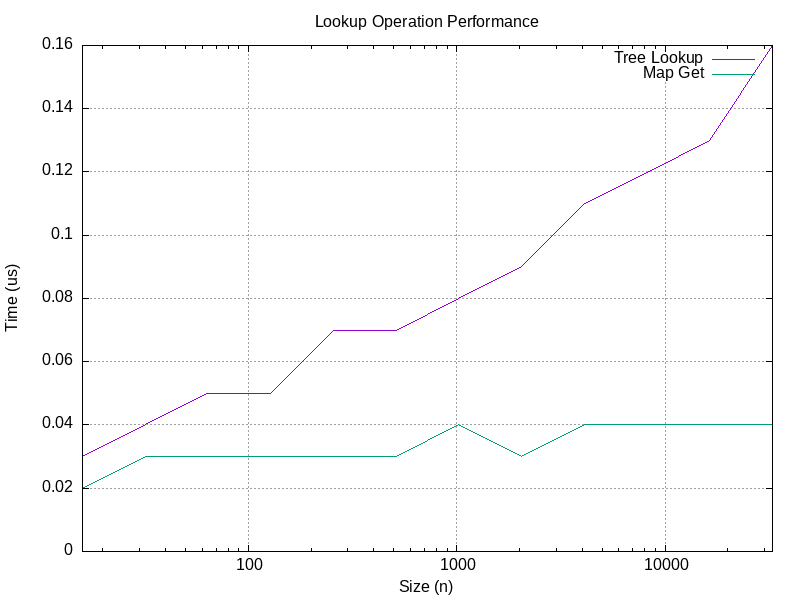
\includegraphics[width=\textwidth]{../data/tm_lookup_performance.png}
    \caption{Lookup Operation Performance, comparing the Tree implementation with the built-in Map}
    \label{fig:tm_lookup_performance}
\end{figure}

\section*{Discussion}
\label{sec:discussion}
    % TODO Svara på alla frågor i pdf:en och gör en analys på benchen.
At worst, a basic BST operation like lookup,
locates a node $n$ in a tree
of height $h$ in $O(h)$ time.
A ''well-balanced'' binary tree will have a height of $(\log n)$,
giving the operations a time complexity of $O(\log n)$.
Since the shape of a BST depend on which order the nodes were
added, it was important for the benchmark to add a random set of keys.
The tree roughly got a height of $\log n$ -- as one can see in the benchmark
result in ~\autoref{fig:tm_lookup_performance} and ~\autoref{tab:performance_metrics_and_ratios_lookup}.

The list-based map performs poorly compared to tree-based map.
Since adding, removing or accessing a value requires one to traverse the list.
The time complexity is therefore linear $O(n)$.

According to
\href{https://hexdocs.pm/elixir/1.12/Map.html}{Elixir official documentation on Maps}
accessing specific keys in the
built-in module work in logarithmic time.
    However, one can read from the benchmark results that the built-in model
    is faster than the tree-based customized implementation that the author wrote.
    The reason for this is that Elixir uses a hash trie data structure,
    implemented in C++ (as mentioned in the instructions:
\href{https://people.kth.se/~johanmon/courses/id1019/seminars/environment/environment.pdf}{'An environment'}).
%https://arunramgt.medium.com/elixir-internal-representation-of-large-maps-hamt-618e1275938d
\end{document}